\documentclass[11pt, a4paper]{article}
\usepackage[letterpaper, portrait, margin=0.5in]{geometry}
\usepackage[english]{babel}  % force American English hyphenation patterns
\usepackage{amsmath,mathtools}

\usepackage{graphicx}
\usepackage{wrapfig}


\begin{document}
\title{Chapter 14 Periodic Motion}
\author{Apostolos Delis}
\date{\today}
\maketitle

\tableofcontents
\section[14.1, Describing Oscillation]{Describing Oscillation}
Oscillation always occurs if the force is a restoring force that
tends to return the system to equilibrium.

\begin{itemize}
    \item In the case of springs, the x component of acceleration is
        \begin{equation*}
            a_x = \frac{F_x}{m}
        \end{equation*}
    \item This force is called the restoring force
\end{itemize}

\subsection{Amplitude, Period, Frequency, and Angular Frequency}
\begin{itemize}
    \item The amplitute of motion (A), is the maximum displacement from the
        equilibrium and is always positive.
    \item The period T represents the time to complete one cycle
    \item The frequency, $f$, is the number of cycles in a unit of time.
    \item The angular frequency $\omega$, is 2$\pi$ times the frequency
        \begin{equation}
        \omega = 2\pi f
        \end{equation}
    \item Additionally, another way of representing period and frequency is
        as reciprocals of eaceh other
        \begin{equation}
            f = \frac{1}{T}
        \end{equation}\break
\end{itemize}
\section[14.2, Simple Harmonic Motion]{Simple Harmonic Motion}
\begin{itemize}
    \item The simplest kind of oscillation occurs when the restoring force Fx is
        directly proportional to the displacement from equilibrium x.
    \item In an ideal spring, the restoring force $F_x$ is equal to $-kx$ where x is
        the displacement and k is the force constant
    \item When the restoring force is proportional to the displacement from equilibrium,
        the oscillation is called simple harmonic motion.
    \item The standard equation for simple harmonic motion is given by:
        \begin{equation}
            a_x = \frac{d^2x}{dt^2} = -\frac{k}{m}x
        \end{equation}
        Where here the $\frac{d^2x}{dt^2}$ is the second derivative of displacement
    \item For many many systems, the restoring force is approximately proportional to
        the displacement, these systems can still be modeled as simple harmonic motion
\end{itemize}
\subsection{Circular motion and the equations of SHM}
\begin{itemize}
    \item In order to explore properties of simple harmonic motion, must express $x$ of the
        oscillating body in terms of time $x(t)$
    \item Phasors are vectors that follow around a body moving in circular motion, these have
        the same angular speed $\omega$ as the rotating body
    \item The x-component of the phasor at time t is just the x-coordinate of the reference
        point $Q$:
        \begin{equation}
            x = Acos\theta
        \end{equation}
        Note that $Q$ is essentially at the origin of the xy plane in this example
    \item The acceleration of $Q$, denoted as $\vec{a}_{Q}$ and is constant. It is
        defined in terms of the angular speed and the radius of the circle
        \begin{equation}
            a_{Q} = \omega{}^2A
        \end{equation}
    \item The equation of angular speed $\omega$ can then be given by
        \begin{equation}
            \omega^{2} = \frac{k}{m} \; \; \; \text{or} \; \; \;  \omega = \sqrt{\frac{k}{m}}
        \end{equation}
    \item Note that we use $\omega$ for both the angular speed at point $Q$ and for the
        angular velocity at point $P$, this is because these quantities are identical
        If point Q makes one complete revolution in time T, then point P goes through
        one complete cycle of oscillation in the same time;
    \item During time $T$, $Q$ moves $2\pi$ radians, so the angular speed is $\omega = 2\pi T$
\end{itemize}
\subsection{Period and amplitude in SHM}
\begin{itemize}
    \item In simple harmonic motion the period and frequency do not depend on the amplitude $A$. The
        reason for this is that the time of one complete oscillation is the same no matter what,
        regardless on the value of $A$.
    \item For a larger $A$, the body reaches $\vert x \vert$ and is thus subjected to larger restoring
        forces, increasing the speed of the body over the cycle, which perfectly compensates for the
        larger travel path
\end{itemize}
\subsection{Displacement, velocity, and acceleration in SHM}
\begin{itemize}
    \item The displacement of simple harmonic motion can be characterized by
        \begin{equation}
            x = A\cos(\omega{}t + \phi)
        \end{equation}
        Where $\phi$ is the phase angle, and the angular frequency is $\sqrt{\frac{k}{m}}$
    \item Variations of simple harmonic motion. All cases shown have $\phi = 0$

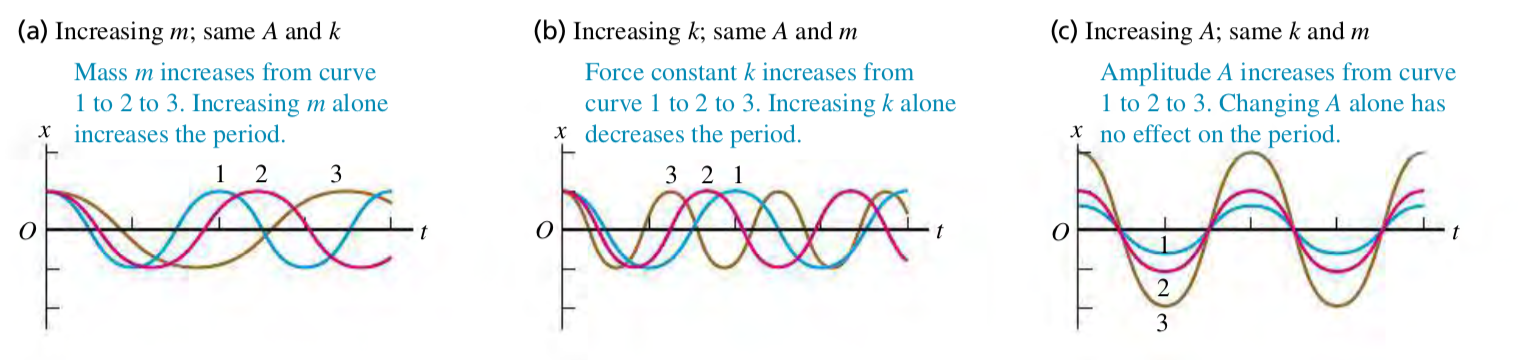
\includegraphics[scale=0.65]{images/shm.png}

    \item If we start at time $t = 0$, then the time $T$ to complete one cycle can be given by
        \begin{equation}
            \omega{}T = \sqrt{\frac{k}{m}}T = 2\pi \; \; \; or \; \; \; T = 2\pi\sqrt{\frac{m}{k}}
        \end{equation}
    \item The velocity and acceleration functions can be calculated as follows
        \begin{equation}
            v_x = \frac{dx}{dt} = -\omega{}A\sin(\omega{}t + \phi)
        \end{equation}
        \begin{equation}
            a_x = \frac{d^2x}{dt^2} = -\omega^{2}A\sin(\omega{}t + \phi)
        \end{equation}
    \item We can then see that from the previous equations:
        \begin{equation}
            a_x = -\omega^{2}x = -\frac{k}{m}x
        \end{equation}
    \item When the body is passing through the equilibrium at x = 0, the velocity equals either
        vmax or -vmax (depending on which way the body is moving) and the acceleration is zero.
    \item When the body is at maximum displacement, $x \pm A$, then the velocity is 0 and the
        magnitute of the acceleration is the largest, and at these points the restoring force is
        $F_x = -kx$
    \item The way to determine the amplitude $A$ and phase angle $f$ for an oscillating body when
        given its initial displacement $x_0$ and initial velocity $v_{0x}$ is to notice that
        \begin{equation}
            v_{0x} = -\omega{}A\sin\phi
        \end{equation}
        To find $\phi$, divide the two equations:
        \begin{equation}
            \frac{v_{0x}}{x_0} = \frac{-\omega{}A\sin\phi}{A\cos\phi} = -\omega\tan\phi
        \end{equation}
        Which then lets us see that
        \begin{equation}
            \phi = \arctan\bigg(-\frac{v_0x}{\omega{}x_0}\bigg)
        \end{equation}
    \item It is also easy to find the amplitude in the previous example, with the following equation
        \begin{equation}
            A = \sqrt{x_{0}^{2} + \frac{v_{0x}^{2}}{\omega^{2}}}
        \end{equation}
\end{itemize}
\section{Energy in Simple Harmonic Motion}
\begin{itemize}
    \item In the rotating body, The vertical forces do no work, so the total mechanical energy of the
        system is conserved.
    \item The kinetic energy of the body is $K = \frac{1}{2}mv^{2}$ and the potential energy of the
    spring is $U = \frac{1}{2}kx^{2}$ So the total mechanical energy is just given by $E = K + U$
    \item Whent the item reaches the point $x = A$, then $v_x = 0$ at this point, so we have that
        \begin{equation}
            E = \frac{1}{2}mv^2 + \frac{1}{2}kx^2 = \frac{1}{2}kA^2 = constant
        \end{equation}
    \item Graphs of E, K, and U versus displacement in SHM.

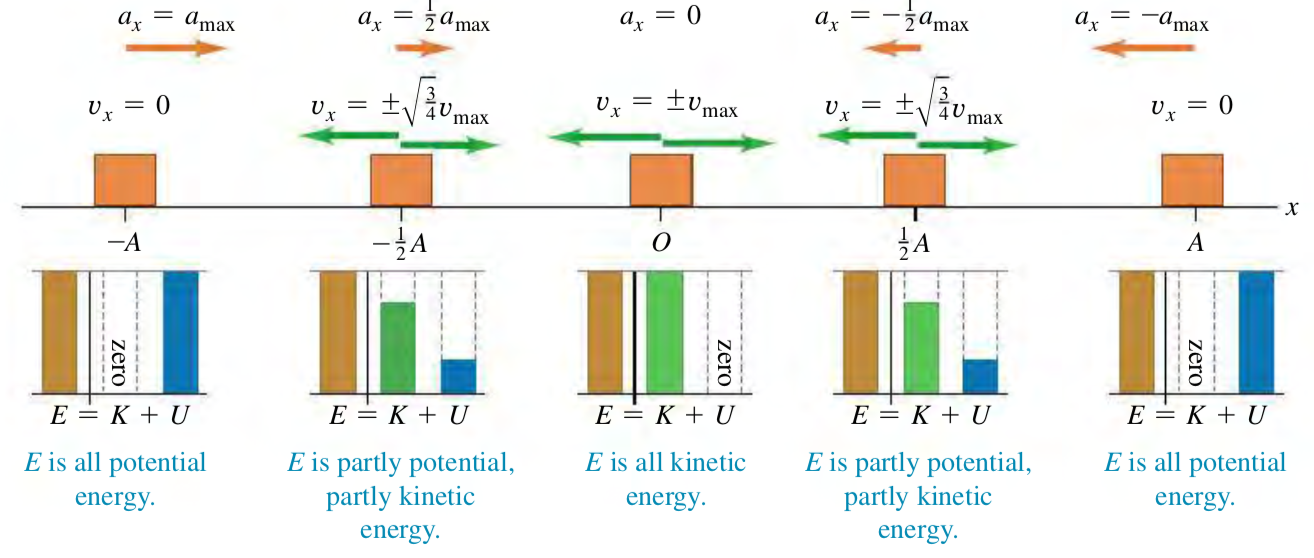
\includegraphics[scale=0.65]{images/eku_plots.png}

    \item This equation can also be verified by plugging in $x$ and $v_x$ as well as using
        $\omega^{2} = \frac{k}{m}$
        \begin{align*}
            E &= \frac{1}{2}mv_{x}^{2} + \frac{1}{2}kx^{2} = \frac{1}{2}m[-\omega
            A\sin(\omega{}t + \phi)]^2 + \frac{1}{2}k[A\cos(\omega{}t + \phi)]^{2}\\
              &= \frac{1}{2}kA^{2}\sin^{2}(\omega t + \phi) + \frac{1}{2}kA^{2}\cos^{2}(
            \omega{}t + \phi) = \frac{1}{2}A^{2}
        \end{align*}
    \item We can also solve for velocity $v_x$ of the body at the given displacement of x
        \begin{equation}
            v_x = \pm \sqrt{\frac{k}{m}}\sqrt{A^{2}-x^{2}}
        \end{equation}
    \item The maximum speed $v_{max}$ occurs at $x = 0$. Using the previous equations and
        $\omega = \sqrt{\frac{k}{m}}$, we have
            \begin{equation}
                v_{max} = \sqrt{\frac{k}{m}}A = \omega{}A
            \end{equation}
            Which agrees that $v_x$ oscillates between $\pm\omega{}A$
\end{itemize}

\section{Applications of Simple Harmonic Motion}
As of now, the only application used has been a body attached to an ideal horizontal spring.
There are however, many different applications of this phenomena, with different restoring
forces for different situations

\subsection{Vertical SHM}
\begin{itemize}
    \item Suppose there is now a vertical spring that is suspended from the ceiling with a
        body attached to it. This spring's equilibrium will be shifted by $\Delta{}l$  such that
        \begin{equation}
            k\Delta{}l = mg = F_g
        \end{equation}
    * When the body is x distance above the equilibrium, the spring is extended
        $\Delta I - x$. Then the upward force exerted is $k(\Delta I - x)$ and the net force is
        \begin{equation}
            F_{net} = k(\Delta I - x) + (-mg) = -kx
        \end{equation}
\end{itemize}
\subsection{Angular SHM}
\begin{itemize}
    \item A mechanical watch which keeps time with a mechanical wheel is an example of angular
        simple harmonic motion. It has a moment of inertia $I$ and a restoring torque $\tau_{z}$
    \item We can write the equation of torque $\tau_{z} = -k\theta$
    \item Using Newton's second law for a rigid body, we have that $\sum\tau_{z} = I\alpha_z =
        I\frac{d^{2}\theta}{dt^{2}}$ and we see that
        \begin{equation}
            -\kappa\theta = I\alpha \; \; \; or \; \; \; \frac{d^{2}\theta}{dt^{2}} =
            -\frac{\kappa}{I}\theta
        \end{equation}
    \item This is exaclty the same equation as for simple harmonic motion but with $x$ replaced
        by $\theta$ and $k/m$ replaced by $\kappa/I$
    \item the angular displacement $\theta$ as a function of time is given by
        \begin{equation}
            \theta = \Theta\cos(\omega{}t + \phi)
        \end{equation}
        Where $\Theta$ is the angular amplitude
\end{itemize}
\section{The Simple Pendulum}
\begin{itemize}
    \item A simple pendulum is an idealized model consisting of a point mass suspended by a
        massless, unstretchable string
    \item The path of the point mass is the arc of a circle with radius L equal to the
        length of the string
    \item The restoring force $F_{\theta}$ is the tangential component of the net force
        \begin{equation}
            F_{\theta} = -mg\sin\theta
        \end{equation}
    \item Gravity provides the restoring force $F_\theta$; the tension T merely acts to
        make the point mass move in an arc,
    \item Since $F_\theta$ is proportional to $\sin\theta$, not to $\theta$, motion is not
        simple harmonic, but for small $\theta$, $\theta \approx \sin\theta$ so it is
        approximately harmonic
    \item With this approximation, it follows that
        \begin{equation}
            F_{\theta} = -mg\theta = -mg\frac{x}{L} = -\frac{mg}{L}x
        \end{equation}
    \item Here the force constant $k$ can be given by $k = mg/L$ and the angular frequency
        $\omega$ with a small amplitude is
        \begin{equation}
            \omega = \sqrt{\frac{k}{m}} = \sqrt{\frac{mg/L}{m}} = \sqrt{\frac{g}{L}}
        \end{equation}
    \item The corresponding frequency and period relationships are
        \begin{equation}
            f = \frac{\omega}{2\pi} = \frac{1}{2\pi}\sqrt{\frac{g}{L}}
        \end{equation}
    \item The motion of the pendulum is only approximately harmonic, for large values of
        angular displacement, $\Theta$, the departures can be modeled as
        \begin{equation}
            T = 2\pi\sqrt{\frac{L}{g}}\bigg(1 + \frac{1^{2}}{2^{2}}\sin^{2}\frac{\Theta}{2}
            + \cdots\bigg)
        \end{equation}
\end{itemize}

\section{The Physical Pendulum}
\begin{itemize}
    \item The physical pendulum is any real pendulum extended body, as contrasted to the
        idealized simple pendulum with all of its mass concentrated at a point.
    \item In equilibrium, the center of gravity is directly below the pivot. When the body
        is displaced as shown, the weight $mg$ causes the restoring torque
        \begin{equation}
            \tau_{z} = -(mg)(d\sin\theta)
        \end{equation}
    \item With a small $\theta \approx \sin\theta$, we have that the torque is
        \begin{equation}
            \tau_{z} = -(mgd)\theta
        \end{equation}
    \item With Newton's Second law, we have that $\sum{}\tau_{z} = I\alpha_{z}$, so
        \begin{equation}
            -(mgd)\theta = I\alpha_{z} = I\frac{d^{2}\theta}{dt^{2}}
        \end{equation}
        \begin{equation}
            \frac{d^{2}\theta}{dt^{2}} = -\frac{mgd}{I}\theta
        \end{equation}
    \item The angular frequency for this is then,
        \begin{equation}
            \omega = \sqrt{\frac{mgd}{I}}
        \end{equation}
        Where $f = (1/2\pi)\omega$ and $T = 1/f$
        \begin{equation}
            T = 2\pi\sqrt{\frac{I}{mgd}}
        \end{equation}
\end{itemize}

\section{Damped Oscillations}
\begin{itemize}
    \item All these oscillations descibed so far however, are frictionless, whereas in the real
        world this is very rarely the case
    \item The decrease in amplitude caused by dissapatitve forces is called damping, which comes as
        a new force $F_{x} = -bv_{x}$ where $v_{x} = dx/dt$ is the velocity and $b$ is the damping
        constant
    \item The net force on the body is then
        \begin{equation}
            \Sigma{}F_{x} = -kx - bv_{x}
        \end{equation}
        with Newton’s second law for the system
        \begin{equation}
            -kx -bv_{x} = ma_{x} \; \; \; or \; \; \; -kx - b\frac{dx}{dt} =
            m\frac{d^{2}x}{dt^{2}}
        \end{equation}
    \item If the damping force is relatively small, the motion is described by
        \begin{equation}
            x = Ae^{-(b/2m)t}\cos(\omega^{\prime}t + \phi)
        \end{equation}
    \item The angular frequency of these damped oscillations is given by
        \begin{equation}
            \omega^{\prime} = \sqrt{\frac{k}{m}-\frac{b^{2}}{4m^{2}}}
        \end{equation}
    \item When $b = 2\sqrt{km}$ the system is said to be critically damped, the system will return
        to equilibrium without oscillating. When $b > 2\sqrt{km}$, the system is said to be
        overdamped, leading to very slow return to equilibrium without oscillating. The solution
        to this system then becomes.
        \begin{equation}
            x = C_{1}e^{-a_{1}t} + C_{2}e^{-a_{2}t}
        \end{equation}
        When $b < 2\sqrt{km}$, the system is overdamed, leading to high oscillation with steadily
        decreasing amplitude
\end{itemize}
\subsection{Energy in Damped Oscillations}
\begin{itemize}
    \item In damped oscillations, the damping force is non-conservative, so the mechanical energy will
        decrease continuously, eventually reaching 0. So start with the derivative of energy:
        \begin{equation}
            \frac{dE}{dt} = mv_{x}\frac{dv_{x}}{dt} + kv\frac{dx}{dt}
        \end{equation}
        But $dv_{x}/dt = a_{x}$ and $dx/dt = v_{x}$ so
        \begin{equation}
            \frac{dE}{dt} = v_{x}(ma_{x} + kx)
        \end{equation}
        Since $ma_{x} + kx = -bdx/dt = -bv_{x}$ so
        \begin{equation}
            \frac{dE}{dt} = v_{x}(-bv_{x}) = -bv_{x}^{2}
        \end{equation}
\end{itemize}
\section{Forced Oscillations and Resonance}
\begin{itemize}
    \item A damped oscillator will eventually stop moving, but its amplitude can be maintained
        if there is a force applied to it in a periodic way. This additional force is called a
        driving force.
    \item The amplitude of a forced oscillator can be found as a function of frequency
        \begin{equation}
            A = \frac{F_{max}}{\sqrt{(k-m\omega^{2}_{d})^{2} + b^{2}\omega_{d}^{2}}}
        \end{equation}
        So from this we can see that $A$ is at its maximum when $\omega_{s} = \sqrt{k/m}$
\end{itemize}

\end{document}
